
\documentclass{article}
\usepackage[utf8]{inputenc}
\usepackage{graphicx}
\graphicspath{ {images/}}
\usepackage{amsthm}
\usepackage{amssymb}
\usepackage{amsfonts}
\usepackage{color}
 \usepackage{wrapfig}

\title{TP 2 \\ Intégration numérique}
\author{SABABADY Kamala et SELVARAJAH Dinusan}

\begin{document}
\maketitle

\section{Partie 1 : $f(x) = \sqrt{1 - x^2}$}

   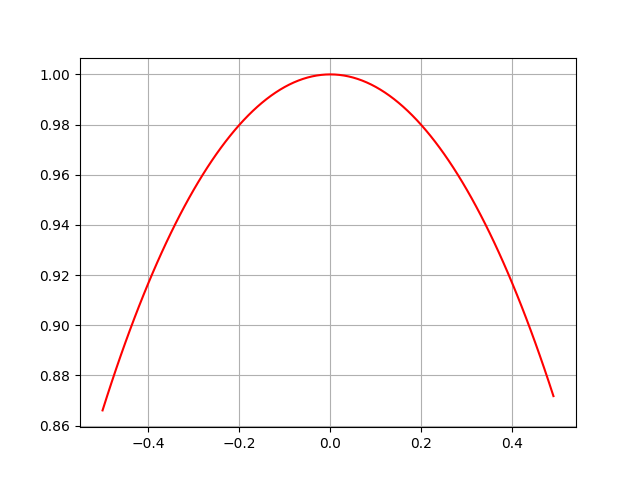
\includegraphics[width=10cm]{1.png}

 	Tout d'abord nous avons définit la fonction $f(x)=\sqrt{1-x^2}$ sous forme d'une fonction Python. Puis nous avons représenter graphiquement f à l'aide de matplotlib.pyplot.


Calculons l'intégrale I de cette fonction sur $[-0.5, 0.5]$ :
$$I=\int_{-0.5}^{0.5} f(x) \, \mathrm{d}x $$
c'est-à-dire : $$I=\int_{-0.5}^{0.5} \sqrt{1-x^2} \, \mathrm{d}x $$
 
On pose $x=sin(y)$ et $\mathrm{d}x=cos(y)\mathrm{d}y$


Donc on a :
$$I=\int_{-\pi/6}^{\pi/6} \sqrt{1-sin(y)^2}*cos(y) \, \mathrm{d}y $$
$$<=> I= \int_{-\pi/6}^{\pi/6} \sqrt{cos(y)^2}*cos(y) \, \mathrm{d}y $$
$$<=> I= \int_{-\pi/6}^{\pi/6} cos(y)*cos(y) \, \mathrm{d}y $$
$$<=> I= \int_{-\pi/6}^{\pi/6} cos(y)^2 \, \mathrm{d}y $$


Or $ cos(y)^2 = \frac{1+cos(2y)}{2}$


Ainsi:
$$ I= \int_{-\pi/6}^{\pi/6} \frac {1+cos(2y)}{2}\, \mathrm{d}y $$
$$ $$
\color{red}
\textbf {La primitive de $\frac{1+cos(2y)}{2}$ est $ I=  [\frac {sin(2y)}{4}\ + \frac {1}{2}*t]$}
\color{black}
\newline
Donc: 
$$ I=  [\frac {sin(2*\pi/6)}{4}\ + \frac {1}{2}*\pi/6]-[\frac {sin(2*(-\pi/6)}{4}\ + \frac {1}{2}*(-\pi/6)]$$
\begin{description}
\item[$<=>$ I =]{$  [\frac {sin(\pi/3)}{4}\ + \pi/12]-[\frac {sin((-\pi/3)}{4}\ + (-\pi/12)]$}
\item[$<=>$ I =]{ $ [\frac {\sqrt{3}/2}{4}\ + \pi/12]-[\frac {(-\sqrt{3}/2)}{4}\ + (-\pi/12)]$}
\item[$<=>$ I =]{$ [\frac {\sqrt{3}/2}{4}\ + \pi/12+\frac {(\sqrt{3}/2)}{4}\ + \pi/12)]$}
\item[$<=>$ I =]{$ {\sqrt{3}/4}\ + \pi/6$}
\end{description}
\textbf {Ainsi l'intégrale de la fonction f est  \color{blue} {$ I= {\sqrt{3}/4}\ + \pi/6 $}}

\section{Partie 2 : Méthode du point milieu}


	
        Nous allons calculer I au moyen de la \textbf{Méthode du point milieu}. Pour cela d'abord on définit une subdivision régulière $x0,x1,...,x4$ de l'intervalle d'intégration $[0,1]$ en n= 4 parts égales puis on définit les milieux de ces sous-intervalles. Avec ces données on calcule la surface $s{k}$ du rectanggle de base $[x{k-1},x{k}]$ et de hauteur $f(c{k})$. On sait que la surface d'un rectangle est $S= b*h$ avec b la base et h la hauteur du rectangle.
	

	Et enfin, on prend la somme $S{4}=\sum_{i=1}^{4} (s_{k})$ comme approximation de I. 
\newline
	\\	Pour calculer l'erreur commise : On soustrait la valeur absolue de $S{4}$ à l'intégrale calculé par la partie 1.
D'après notre programme qui permet de calculer $S{k}$, nous avons trouvé l'erreur commise: $$\vert S_4 - I \vert = 0.724855274769$$
\newline
         Puis nous avons utilisé la fonction \textit {clock()} du module time pour mesurer le temps de calcul de notre intégrale.
Et nous avons trouvé $t= ...$.
\newline
\\

	Afin de calculer l'intégrale I de la fonction f pour un entier n quelconque, on a définit une fonction python \textit{point\_milieu} qui prend en arguments une fonction f, des bornes a,b et un entier n et qui renvoie l'intégrale approchée de f sur $[a,b]$ au moyen du point milieu. 
	\\
\\
	Nous avons pas eu de difficulté pour cette fonction puisqu'on l'a faite pour n=4.
\\
Ensuite, on a testé notre programme avec $f(x)= \sqrt{1 - x^2}$, $a=-0.5 $,$b=0.5$ et $ n=10^{k}$, k variant de 1 à 6 ce qui nous a permit de remplir le tableau ci-dessous:
\\

\begin{center}
\begin{tabular}{r | c | c}
{n} & erreur & temps (sec.)\\
\hline
$10$ & {0.000480383653956} & {7.7e-05}\\
$100$ & {4.81117740869e-06} & {0.000499}\\
$1000$ & {4.811251475e-08} & {0.003855}\\
$10000$ & {4.81136575026e-10} & {0.01302}\\
$100000$ & {4.75719463822e-12} & {0.119425}\\
$1000000$ & {7.64943663967e-13} & {1.165697}
\end{tabular}
\end{center}

Ensuite, on a essayé d'afficher ce tableau à l'écran (sur le terminal), mais au début on n'a pas eu d'idée et on ne savait pas comment le faire, après des recherches sur internet , on a réussi à afficher ce tableau à l'écran.

\section{Partie 3 : Méthode du trapèze}


	Pour la\textbf { méthode du trapèze}, on approxime f sur l'intervalle $[x{k-1},x{k}]$ par la fonction affine qui prend les mêmes valeurs que f en $x_{k-1}$ et $x_k$.\\

	On a essayé de calculer approché de I par la méthode du trapèze. Pour cela d'abord, on définit la fonction \textit{trapeze} qui prend en arguments une fonction f, des bornes a, b et un entier n et qui renvoie l'intégrale approchée de f sur $[a,b]$ au moyen de la méthode du trapèze.\\

	Puis on a testé avec $f(x)= \sqrt{1 - x^2}$, $a=-0.5 $,$b=0.5$ et $ n=10^{k}$, k variant de 1 à 6 et on a utilisé la fonction \textit{clock()} pour mesurer le temps de calcul de notre programme. \\ On a également calculer l'erreur commise $\vert S - I \vert $ avec S l'intégrale calculé par notre fonction \textit{trapezes} et I l'intégrale calculé à la partie 1. \\ 

Avec ces données nous avons rempli le tableau ci-dessous:


\begin{center}
\begin{tabular}{r | c | c}
{n} & erreur & temps (sec.)\\
\hline
$10$ & {0.000961402186473} & {2.39999999998e-05}\\
$100$ & {9.62241895941e-06} & {0.000112}\\
$1000$ & {9.62250357173e-08} & {0.001087}\\
$10000$ & {9.62250168435e-10} & {0.011264}\\
$100000$ & {9.63307211777e-12} & {0.103774}\\
$1000000$ & {1.11022302463e-13} & {0.770158}
\end{tabular}
\end{center}

\section{Partie 4 : Méthode de Simpson}
\begin{center}

\includegraphics[width=0.25\textwidth]{doc1.jpeg}

\includegraphics[width=0.25\textwidth]{rir.jpg}
\end{center}
Pour la méthode de Simpson, on approxime f sur l'intervalle $[x_{k-1}, x_k]$ par le polynôme de degré 2 qui prend les mêmes valeurs que f en $x_{k-1}$, $c_k$ et $x_k$.\\
Nous avons définit la fonction Simpson à l'aide d'un site expliquant la méthode et cela n'a pas été un probléme. Puis nous avons testé notre programmme avec $f(x)= \sqrt{1 - x^2}$, $a=-0.5 $,$b=0.5$ et $ n=10^{k}$, k variant de 1 à 6 et comme pour les autres programme, nous avons utilisé la fonction \textit{clock()}. Donc avec ces données, nous avons rempli le tableau ci-dessous: \\

\begin{center}
\begin{tabular}{r | c | c}
{n} & erreur & temps (sec.)\\
\hline
$10$ & {2.1162618713e-07} & {0.000153000000001}\\
$100$ & {2.13807860305e-11 } & {0.000768000000001}\\
$1000$ & {1.55431223448e-15} & {0.008067}\\
$10000$ & {2.6645352591e-15} & {0.046923}\\
$100000$ & {9.99200722163e-16} & {0.16951}\\
$1000000$ & {2.17603712827e-14} & {1.676945}
\end{tabular}
\end{center}

\section{Partie 5 : Comparaison des trois méthodes précédentes }

Les trois méthodes : \textbf {Méthode du Point\_Milieu, Méthode du Trapèze, Méthode de Simpson} nous permettent de calculer une approximation d'intégrale d'une fonction sur un intervalle. 
\\

	
	Les différences entre ces méthodes sont que : dans la \textit{méthode du point milieu} on approxime f par la fonction constante , dans la \textit{méthode du Trapèze} on approxime par la fonction affine et dans la \textit{méthode de Simpson} on approxime par la fonction du polynôme de degré 2. 
\\

	On remarque que l'erreur commise pour chaque méthodes sont différentes. On voit que la méthode de Simpson est plus efficace que les deux autres méthodes puisque les erreurs commises par la méthode de Simpson sont très inférieurs à ceux des deux autres méthodes.


\section{Partie 6 : Méthode de Monte-Carlo}

Pour dessiner le cercle on y a pris du temps car on ne savait pas la fonction qui fallait utiliser sur Python, suite à plusieurs essais et plusieurs recherches sur internet on a réussi à le faire. Voici le cercle tracé :

\begin{wrapfigure}{l}{0.65\textwidth}
    \centering
    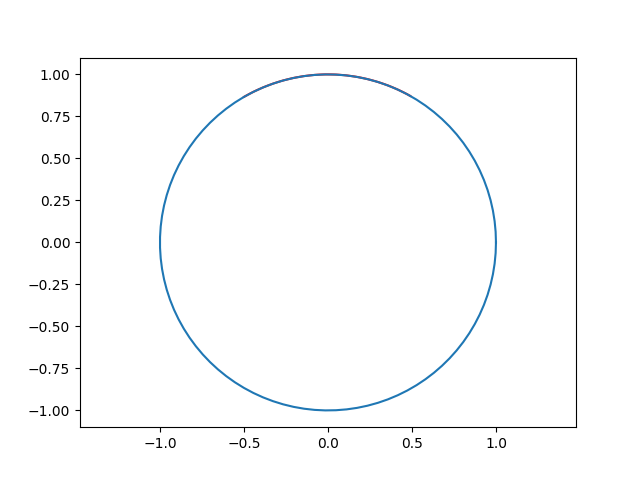
\includegraphics[width=0.65\textwidth]{cercle.png}
\end{wrapfigure}
$$ $$
$$ $$
$$ $$
La surface du disque à l'unité est $\pi$.
$$ $$
$$ $$
$$ $$
$$ $$
$$ $$
Grâce à la fonction \textit{numpy.random.rand()}, on a généré quelques valeurs aléatoire suivant la distribution de la loi uniforme sur $[0,1]$ et sur $[-1,1]$.
\\
Puis on génére 1000 points suivants la distribution uniforme sur le carré $[-1,1]^2$ et on a fait apparaître sur le graphique précédent les points inférieurs au disque unité en rouge et les points extérieurs au disque en vert. Voici le graphique:\\
	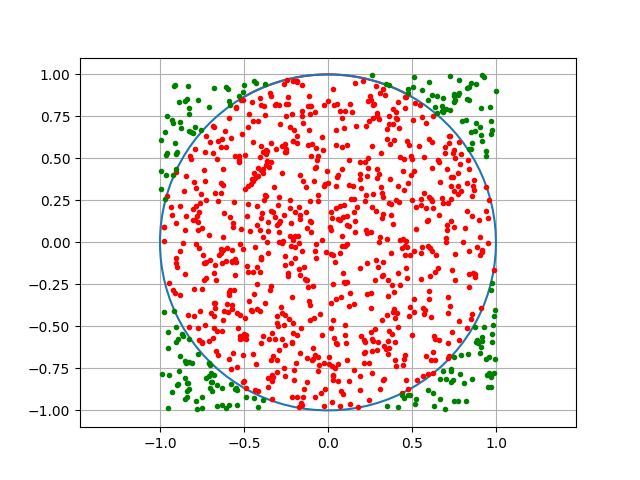
\includegraphics[width=0.65\textwidth]{rougevert.png}

Ensuite on a compté le nombre I de points intérieurs et le nombre E de points extérieurs. \\ On sait que la méthode de Monte Carlo consiste à prendre le rapport $\frac{I}{N}$ comme approximation de la surface S du disque. Ainsi nous avons calculé la valeur absolue du rapport $\frac{I}{N}$ soustrait à S pour savoir l'erreur commise par la fonction Monte Carlo. On a utilisé time.clock() pour mesurer le temps de calcul de ce calcul.
\\
On a testé la fonction \textit{Monte\_Carlo} avec $N=10^k$, k variant de 1 à 6 puis on a enregistré dans un fichier texte. Mais pour enregistrer dans un fichier on a eu un peu de difficulté car au début on ne savait pas comment le faire, après l'aide d'un ami on a réussi a le faire.\\
Monte Carlo est une fonction avec des valeurs aléatoire donc on n'a pas pu remplir le tableau puisqu'il change à chaque fois (voir montecarlo.txt).\\

Et enfin, on a définit une fonction \textit{monte\_carlo\_2} pour le calcul du volume de la boule unité.  


\end{document}
